\documentclass[11pt]{article}
\usepackage[margin=1in]{geometry}
\usepackage{amsmath,amssymb,amsthm,booktabs,graphicx,hyperref}
\hypersetup{colorlinks=true,urlcolor=blue,linkcolor=blue,citecolor=blue,pdftitle={Certified numerical inputs for a selected Einstein-scalar shell perturbation},pdfauthor={Ricardo Maldonado}}
\newtheorem{proposition}{Proposition}
\newcommand{\Ev}{E_v}
\title{Certified numerical inputs and a sharp angular evaluation bound\\for a selected Einstein--scalar shell perturbation}
\author{Ricardo Maldonado\\Independent Researcher\\Henderson, Nevada, United States}
\date{October 2026}
\begin{document}
\maketitle
\begin{abstract}
We prepare the numerical evaluation of a previously constructed conditional formal second-order Einstein--scalar perturbation with a timelike material shell. For one aligned quadrupole, the selected quadratic angular feature space admits the sharp evaluation constant $\sqrt{321/19}$. Differentiated integral equations give continuous scaled third-jet errors for explicit first-master and gauge approximations. Whole-cell rational interval evaluation encloses the selected second initial profiles, and tightens the inherited global second-response norm bound to $1.03\times10^{33}$. This is an upper bound for a formal coefficient, not a computed waveform or finite-amplitude nonlinear estimate. The actual quadratic bulk forcing and a continuous numerical second-response residual still require evaluation.
\end{abstract}

\section{Retained problem and conventions}
The parent construction and sources are available at \url{https://github.com/maldonado-research/HDblast/tree/main/research/HDBLAST_COMMON_GAUGE_FORCING_20261016}. This is a computational working note, with no accompanying journal submission.

The retained smooth regular background, fixed scalar potential and shell tension, actual first master and relative-harmonic gauge solutions, and chosen second initial prescription are premises. We use
\[
\ell=10^{-6},\qquad x=t/\ell,\quad r=z/\ell,\qquad
\mathcal D=\{0\le x\le3,\ r\ge0,\ x+r\le8\}\times S^3,
\]
with $dy=-\rho\,dz$ and two identical copy-even interiors. Expansions use $g_\epsilon=g_0+\epsilon q+\epsilon^2 k/2$ and the same factorial convention for the scalar. $H$ denotes probability-normalized angular $L^2$ with positive Frobenius metric pairing. The accepted causal equation is
\[
U=b+TU,\quad b=U_{\rm free}+KF+LG,\quad
TU=K(AU_x+BU_r+DU)+L(MU|_{r=0}),
\]
where $K$ is the mixed reflected wave integral and $L$ the Neumann lift. In
\[
\|U\|_X=\max\{\sup|U|_H/3,\sup|U_x|_H,\sup|U_r|_H\},
\quad\|T\|\le q=0.002109<1,
\]
the formal solution is $\sum_{j\ge0}T^jb$. Its natural bulk equations, physical shell rows, compatible initial data and subsidiary constraints were addressed in the parent checkpoint. No exact nonlinear family is inferred.

\section{Selected angular space and pointwise evaluation}
Fix $Y=n_1^2-n_2^2$, $S=n_1^2+n_2^2$ and
\[
Z=S-\tfrac12,\qquad F_4=Y^2-S/2+\tfrac1{12}.
\]
The multiplicity-free decomposition of the symmetric square of the degree-two scalar representation is
\[
\operatorname{Sym}^2(1,1)=(0,0)\oplus(1,1)\oplus(2,2)\oplus(2,0)\oplus(0,2).
\]
Their section multiplicities are $5,8,8,1,1$. Equivariant quadratic maps evaluated at the same selected first state therefore lie in a 23-dimensional feature space $\Ev$. It has five copies of $1,Z,F_4$, two copies of $DZ,DF_4$, and the tensor features
\[
(D^2Z)^{\rm TF},\quad(D^2F_4)^{\rm TF},\quad T_+,\quad T_-.
\]
Both chiral TT features are retained. This restriction follows from quadratic origin and equivariance, not from the state stabilizer alone. Arbitrary extra second initial data need not satisfy it. The selected initial prescription, natural source maps, bulk operator, boundary maps and causal propagators preserve it.

\begin{proposition}
For the selected feature space, with the stated Frobenius norm and probability sphere measure,
\[
|U(n)|_F\le C_*\|U\|_H,\qquad C_*^2=321/19.
\]
The constant is sharp. The full 287-section space retains its previous bound; a feature count alone does not supply an evaluation constant.
\end{proposition}
\begin{proof}
The three scalar squared norms are $1,1/12,19/720$; the two gradient squared norms are $2/3,19/30$; the four tensor squared norms are $20/9,133/15,1/6,1/6$. Orthogonality between physical scalar, vector and trace-free tensor output blocks makes the evaluation operator block diagonal. Repeated physical copies do not multiply its operator norm. The scalar kernel is
\[
K_s=1+12Z^2+(720/19)F_4^2.
\]
On $X=n_1^2\ge0$, $W=n_2^2\ge0$, $X+W\le1$, exact triangle Bernstein reconstructions bound $K_s$ by $321/19$, the vector block trace by $320/19$, and the tensor block trace by $7698/665$. All coefficients and reconstruction identities are rational; the separate checker records them. The latter two trace bounds also bound their respective operator norms. At $n=e_1$, the scalar reproducing vector is $1+6Z+(420/19)F_4$. Its squared evaluation-to-$L^2$ ratio is $321/19$, proving sharpness.
\end{proof}
The standard $S^3$ harmonic identities supply an independent normalization and eigenvalue comparison~\cite{LTZ}. The proof above is an explicit selected-space calculation. We may use $C_*<4.111$ for values and scaled $x,r$ derivatives that stay in $\Ev$.

\section{Actual first-field approximation errors}
Let $Q$ be the registered unit-height smooth packet on $1<r<2$, with flat zero extension. Put $Q_o(s)=\operatorname{sgn}(s)Q(|s|)$ and $P_e(s)=sQ(|s|)$. Explicit comparison functions are
\[
\overline W(x,r)=\tfrac12[Q_o(r+x)+Q_o(r-x)],
\]
\[
\overline\xi=(P,0,0),\quad P=\frac c4\{P_e(r+x)+P_e(r-x)
-r[Q_o(r+x)+Q_o(r-x)]\},\qquad c=6\ell/130.
\]
The first is displacement-only: the actual nonzero initial velocity and its radial jets remain in the error. The gauge comparison has zero initial value and velocity, the required homogeneous shell rows, and satisfies its explicit forced wave identity. The true master dynamic boundary trace is retained.

For each total scaled derivative order $j$, differentiating the true reflected integral equations bounds the actual master error by the sum of its initial-velocity, dynamic boundary-lift and Duhamel-source errors. Conservative decimal bounds are
\[
\max_{i+k=j}\|\partial_x^i\partial_r^k(W-\overline W)\|_\infty
<\begin{cases}
1.93\times10^{-4},&j=0,\\
4.88\times10^{-4},&j=1,\\
2.09\times10^{-3},&j=2,\\
0.125,&j=3.
\end{cases}
\]
The gauge error is treated through the actual differentiated residual system and a positive matrix resolvent. Nonzero stabilized third initial jets, coefficient derivatives, reflected transitions and radial residual recovery are included. Its complete exact mixed-jet bounds and the correlated affine background approximation through scaled radial order four are in the executable reports. No derivative error is obtained by differentiating a $C^0$ error bound.

\section{Initial profiles and the refined response majorant}
The selected physical second initial data solve the differentiated Hamiltonian and momentum constraints by the retained explicit scalar-sector compensators. Their lapse square, mixed gauge-velocity conversion, nonzero second scalar and scalar velocity are preserved. Shared functional expressions cancel analytically before interval evaluation. A complete annulus partition and analytic flat-endpoint tails enclose all profiles over the entire initial sphere; rational exponential bounds and outward-rounded interval jets control evaluation. These are whole-cell enclosures, not point samples or an interpolation error certificate.

Let $g_0,g_r,g_x$ bound every initial metric frame component and its scaled radial and time partial derivatives, and let $w_0,w_r,w_x$ be the scalar bounds. Then
\[
u_0=5g_0+w_0,\quad u_r=5g_r+w_r,\quad u_x=5g_x+w_x,
\qquad B_{\rm free}=\max\{u_0/3+u_x,u_r+u_x\}.
\]
The factor five follows from the positive Frobenius norm of a symmetric $5\times5$ tensor. Keeping the parent bulk and shell source bounds unchanged gives
\[
\|U\|_X\le\frac{B_{\rm free}+3F_H+G_H}{1-q}<1.03\times10^{33}.
\]
This is about 990 times smaller than the former rounded $1.02\times10^{36}$ bound. It tightens a conservative majorant; it does not measure the actual response. In the selected space,
\[
\sup|U|_F<1.270299\times10^{34},\qquad
\sup|U_x|_F,\sup|U_r|_F<4.23433\times10^{33}.
\]
The companion exact join authenticates every input and verifies these strict rounded inequalities.

The actual initial scalar mean is positive on $[73/64,585/512]$ and negative on $[951/512,119/64]$, with magnitude exceeding $7\times10^{30}$ on both complete cells. Six ordered alternating signed cells give at least five distinct interior zeros by continuity. These concern the selected initial coefficient, not the earlier coordinate shell sources or an evolved waveform. The second initial prescription is not unique; neither these large coefficients nor tightened upper bounds establish physical instability.
\begin{figure}[htbp]
\centering
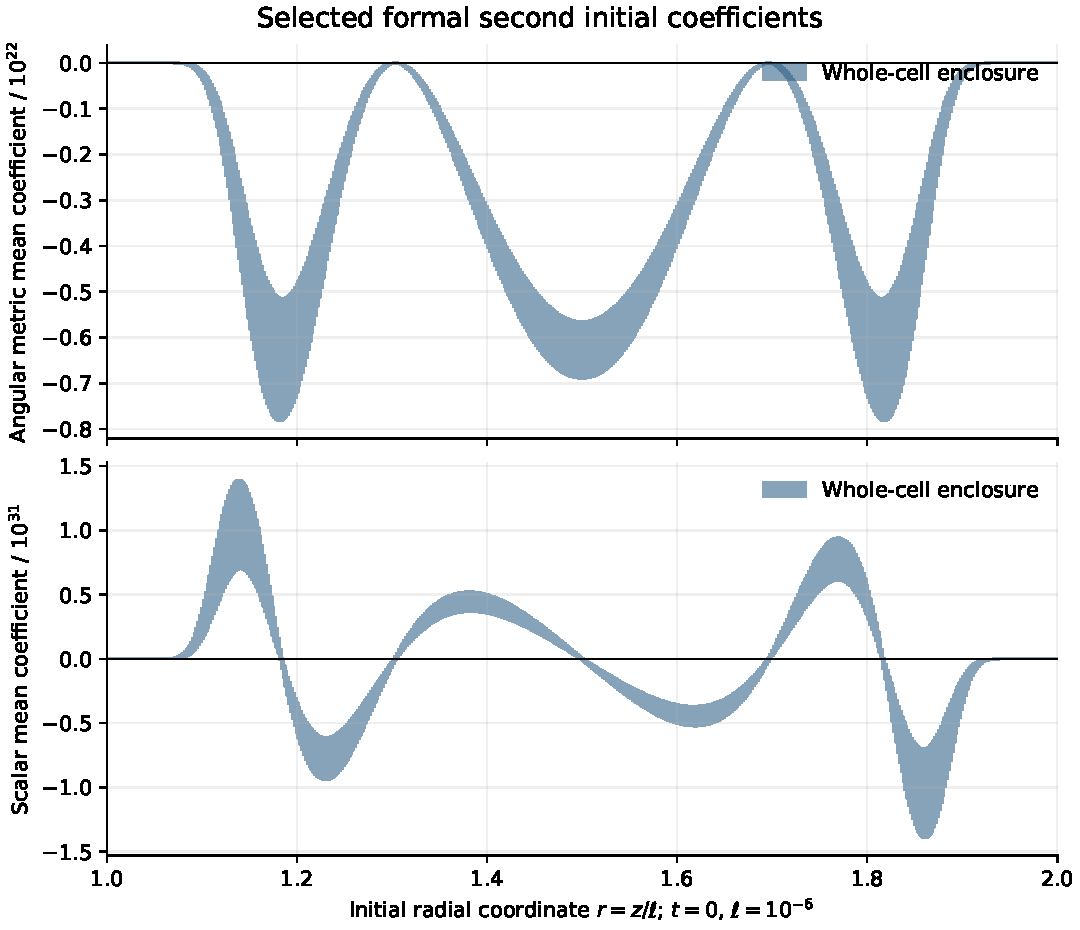
\includegraphics[width=.91\linewidth]{figures/INITIAL_PROFILE_ENCLOSURES.pdf}
\caption{Whole-cell enclosures of selected formal second initial coefficients. Each band encloses all points in its radial cell; plotting uses display-only floating-point conversion. The scalar curve is the probability-normalized angular mean. These are second parameter derivatives, not physical forces or a computed second-order evolution.}
\end{figure}

\section{Remaining numerical and physical questions}
A continuous numerical response still requires the actual transformed two-jets, quadratic bulk and shell source errors, angular source projections, quadrature/reconstruction error and the complete residual on causal cells and shell transitions. For a reconstructed candidate $V$, the retained estimate is
\[
\|U-V\|_X\le\frac{\|V-b-TV\|_X}{1-q}.
\]
First-field approximation certificates are inputs to this estimate; they are not its completed second-response residual. Recent wave reconstruction work motivates explicit separation of input, reconstruction and discretization errors~\cite{DMW,DGMW}, but its scalar Dirichlet displacement estimates do not directly control this mixed-shell norm or third jets. Shell geometry and embedding must transform together when defining a physical observation~\cite{Mars}.

The present results concern a selected perturbative coefficient and registered gauge. No numerical waveform, invariant force, finite-amplitude nonlinear remainder, external novelty, journal acceptance or higher-dimensional origin of the Big Bang is established. Independent checks are internal computational reviews, not external specialist peer review. The frozen parent manuscript is unchanged.

\begin{thebibliography}{9}
\bibitem{LTZ} L.~Lindblom, N.~W.~Taylor and F.~Zhang, \emph{Scalar, Vector and Tensor Harmonics on the Three-Sphere}, Gen. Relativ. Gravit. 49, 139 (2017), \href{https://arxiv.org/abs/1709.08020v1}{arXiv:1709.08020v1}.
\bibitem{DMW} Z.~Dong, L.~Mascotto and Z.~Wang, \emph{A priori and a posteriori error estimates of a C0-in-time method for the wave equation in second order formulation}, \href{https://arxiv.org/abs/2411.03264v3}{arXiv:2411.03264v3}.
\bibitem{DGMW} Z.~Dong, E.~H.~Georgoulis, L.~Mascotto and Z.~Wang, \emph{A posteriori error analysis and adaptivity of a space-time finite element method for the wave equation in second order formulation}, \href{https://arxiv.org/abs/2509.08537v2}{arXiv:2509.08537v2}.
\bibitem{Mars} M.~Mars, \emph{First and Second Order Perturbations of Hypersurfaces}, Class. Quantum Grav. 22, 3325 (2005), \href{https://arxiv.org/abs/gr-qc/0507005v1}{gr-qc/0507005v1}.
\end{thebibliography}
\end{document}
